\documentclass[tikz,border=10pt]{standalone}
\usepackage{pgfplots}
\pgfplotsset{compat=1.18}

\begin{document}

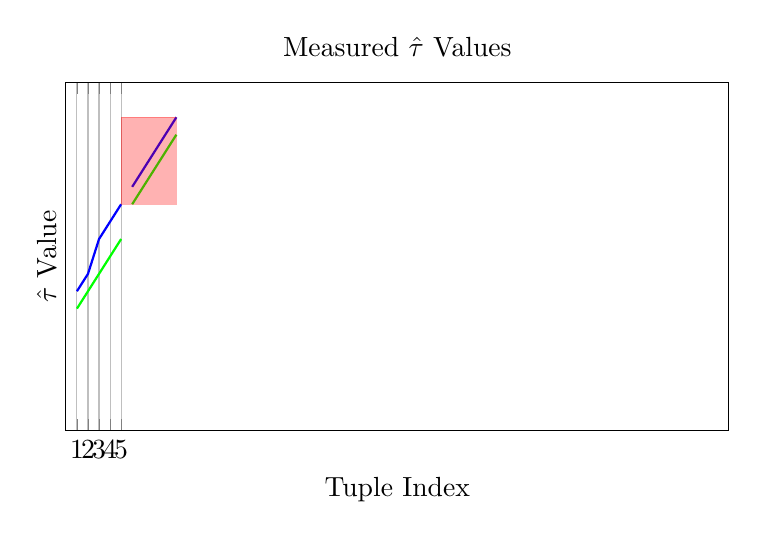
\begin{tikzpicture}
    \begin{axis}[
        title={Measured $\hat{\tau}$ Values},
        xlabel={Tuple Index},
        ylabel={$\hat{\tau}$ Value},
        xmin=0,
        xmax=60,
        ymin=0,
        ymax=2,
        ytick=\empty,
        xtick=data,
        grid=major,
        width=10cm,
        height=6cm
    ]
        
        % Sample data points (replace these with actual data)
        \addplot[blue, thick] coordinates {(1, 0.8) (2, 0.9) (3, 1.1) (4, 1.2) (5, 1.3)};
        \addplot[green, thick] coordinates {(1, 0.7) (2, 0.8) (3, 0.9) (4, 1.0) (5, 1.1)};
        
        % Additional data points for clarity
        \addplot[blue, thick] coordinates {(6, 1.4) (7, 1.5) (8, 1.6) (9, 1.7) (10, 1.8)};
        \addplot[green, thick] coordinates {(6, 1.3) (7, 1.4) (8, 1.5) (9, 1.6) (10, 1.7)};
        
        % Highlighting where blue curve surpasses green
        \filldraw[red, opacity=0.3] (5, 1.3) rectangle (10, 1.8);
        
    \end{axis}
\end{tikzpicture}

\end{document}